\documentclass[12pt]{article}
\usepackage{fullpage,enumitem,amsmath,amssymb,graphicx,booktabs}
\usepackage{sectsty}
\usepackage{float}
\usepackage{parskip}
\sectionfont{\fontsize{15}{20}\selectfont}


\DeclareMathOperator*{\argmax}{arg\,max}
\DeclareMathOperator*{\argmin}{arg\,min}
\DeclareMathOperator{\E}{\mathbb{E}}
\newcommand{\dataset}{\mathcal{D}}
\newcommand{\task}{\mathcal{T}}
\newcommand{\supportdata}{\mathcal{D}^\mathrm{tr}}
\newcommand{\querydata}{\mathcal{D}^\mathrm{ts}}
\newcommand{\support}[1]{{#1}^\mathrm{tr}}
\newcommand{\query}[1]{{#1}^\mathrm{ts}}
\usepackage{bbm}
\usepackage{gensymb}
\usepackage{xcolor}

\usepackage{tgpagella}

\begin{document}

\begin{center}
{{\Large \textbf{CS 330 Autumn 2022 Homework 2 \\ Prototypical Networks and Model-Agnostic Meta-Learning}}
\\ {\large Due Monday October 24, 11:59 PM PST}}

\begin{tabular}{rl}
SUNet ID: &  \\
Name: &Seok, Jeongeum\\
Collaborators: & 
\end{tabular}
\end{center}

By turning in this assignment, I agree by the Stanford honor code and declare that all of this is my own work.

\section*{Overview}

In this assignment, you will experiment with two meta-learning algorithms, prototypical networks (protonets)~\cite{prototypical} and model-agnostic meta-learning (MAML)~\cite{maml}, for few-shot image classification on the Omniglot dataset \cite{Lake1332}, which you also used for Homework 1. You will:
\begin{enumerate}
    \item Implement both algorithms (given starter code).
    \item Interpret key metrics of both algorithms.
    \item Investigate the effect of task composition during protonet training on evaluation.
    \item Investigate the effect of different inner loop adaptation settings in MAML.
    \item Investigate the performance of both algorithms on meta-test tasks that have more support data than training tasks do.
\end{enumerate}

\section*{Expectations}
\begin{itemize}
    \item We expect you to develop your solutions locally (i.e. make sure your model can run for a few training iterations), but to use GPU-accelerated training (e.g. Azure) for your results.
    \item Submit to Gradescope
    \begin{enumerate}
        \item a \texttt{.zip} file containing your modified version of \texttt{hw2/starter/}
        \item a \texttt{.pdf} report containing your responses
    \end{enumerate}
    \item You are welcome to use TensorBoard screenshots for your plots. Ensure that individual lines are labeled, e.g. using a custom legend, or by text in the figure caption.
    \item Figures and tables should be numbered and captioned.
\end{itemize}


\newpage
\section*{Preliminaries}
\textbf{Notation}
\begin{itemize}
    \item $x$: Omniglot image
    \item $y$: class label
    \item $N$ (way): number of classes in a task
    \item $K$ (shot): number of support examples per class
    \item $Q$: number of query examples per class
    \item $c_n$: prototype of class $n$
    \item $f_\theta$: neural network parameterized by $\theta$
    \item $\task_i$: task $i$
    \item $\supportdata_i$: support data in task $i$
    \item $\querydata_i$: query data in task $i$
    \item $B$: number of tasks in a batch
    \item $\mathcal{J}(\theta)$: objective function parameterized by $\theta$
\end{itemize}




\newpage
\section*{Part 1: Prototypical Networks (Protonets)~\cite{prototypical}}

\subsubsection*{Algorithm Overview}
\begin{figure}[H]
\centering
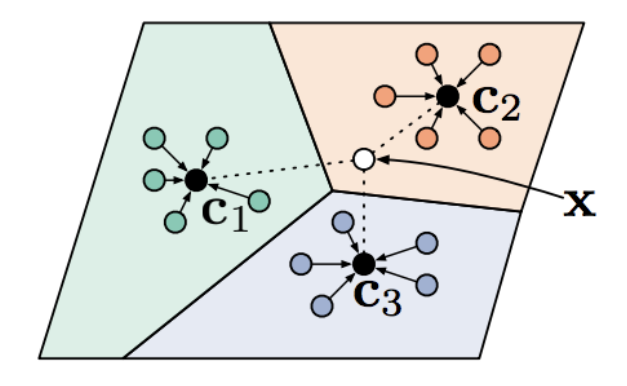
\includegraphics[width=0.5\linewidth]{figures/protonets.png}
\vspace{-3mm}
\caption{Prototypical networks in a nutshell. In a 3-way 5-shot classification task, the class prototypes $c_1, c_2, c_3$ are computed from each class's support features (colored circles). The prototypes define decision boundaries based on Euclidean distance. A query example $x$ is determined to be class 2 since its features (white circle) lie within that class's decision region.}
\label{fig:protonet}
\end{figure}

As discussed in lecture, the basic idea of protonets is to learn a mapping $f_\theta(\cdot)$ from images to features such that images of the same class are close to each other in feature space. Central to this is the notion of a \emph{prototype}
\begin{equation}
    c_n = \frac{1}{K} \sum_{(x,y) \in \supportdata_i : y = n} f_\theta(x),
\end{equation}
i.e. for task $i$, the prototype of the $n$-th class $c_n$ is defined as the mean of the $K$ feature vectors of that class's support images.
To classify some image $x$, we compute a measure of distance $d$ between $f_\theta(x)$ and each of the prototypes. We will use the squared Euclidean distance:
\begin{equation}
    d(f_\theta(x), c_n) = \lVert f_\theta(x) - c_n \rVert_2^2.
\end{equation}
We interpret the negative squared distances as logits, or unnormalized log-probabilities, of $x$ belonging to each class. To obtain the proper probabilities, we apply the softmax operation:
\begin{equation}
    p_\theta(y=n|x) = \frac{\exp(-d(f_\theta(x), c_n))}{\sum_{n'=1}^N \exp(-d(f_\theta(x), c_{n'}))}.
\end{equation}
Because the softmax operation preserves ordering, the class whose prototype is closest to $f_\theta(x)$ is naturally interpreted as the most likely class for $x$. To train the model to generalize, we compute prototypes using support data, but minimize the negative log likelihood of the query data
\begin{equation}
    \mathcal{J}(\theta) = \E_{\task_i \sim p(\task), (\supportdata_i, \querydata_i) \sim \task_i} \left[ \frac{1}{NQ} \sum_{(\query{x},\query{y}) \in \querydata_i} - \log p_\theta(y = \query{y} | \query{x}) \right].
    \label{eq:protonet_objective}
\end{equation}

Notice that this is equivalent to using a cross-entropy loss.

We optimize $\theta$ using Adam~\cite{kingma2014adam}, an off-the-shelf gradient-based optimization algorithm.
As is standard for stochastic gradient methods, we approximate the objective~\eqref{eq:protonet_objective} with Monte Carlo estimation on minibatches of tasks. For one minibatch with $B$ tasks, we have

\begin{equation}
    \mathcal{J}(\theta) \approx \frac{1}{B} \sum_{i=1}^B 
     \left[ \frac{1}{NQ} \sum_{(\query{x},\query{y}) \in \querydata_i} - \log p_\theta(y = \query{y} | \query{x}) \right].
    \label{eq:protonet_objective_minibatch}
\end{equation}


\subsubsection*{Problems}


\begin{enumerate}
    \item We have provided you with \texttt{omniglot.py}, which contains code for task construction and data loading.
    \begin{enumerate}[label=(\alph*)]
        \item (5 pt) Recall that for training black-box meta-learners in the previous homework we needed to shuffle the query examples in each task. This is not necessary for training protonets. Explain why.
        
        \textcolor{red}{Shuffling examples does not change the prototype since it is represented as sum which is commutative.}
        
    \end{enumerate}
    
    \newpage
    \item In the \texttt{protonet.py} file, complete the implementation of the \texttt{ProtoNet.\_step} method, which computes \eqref{eq:protonet_objective_minibatch} along with accuracy metrics. Pay attention to the inline comments and docstrings.
    
    Assess your implementation on 5-way 5-shot Omniglot. To do so, run 
    \begin{equation*} 
        \texttt{python protonet.py} 
    \end{equation*}
    with the appropriate command line arguments. These arguments have defaults specified in the file. To specify a non-default value for an argument, use the following syntax:
    \begin{equation*}
        \texttt{python protonet.py --argument1 value1 --argument2 value2}
    \end{equation*}
    Use 15 query examples per class per task. Depending on how much memory your GPU has, you may want to adjust the batch size. Do not adjust the learning rate from its default of $0.001$.
    
     As the model trains, model checkpoints and TensorBoard logs are periodically saved to a \texttt{log\_dir}. The default \texttt{log\_dir} is formatted from the arguments, but this can be overriden. You can visualize logged metrics by running
    \begin{equation*}
        \texttt{tensorboard --logdir logs/}
    \end{equation*}
    and navigating to the displayed URL in a browser. If you are running on a remote computer with server capabilities, use the \texttt{--bind\_all} option to expose the web app to the network. Alternatively, consult the Azure guide for an example of how to tunnel/port-forward via SSH.
    
    To resume training a model starting from a checkpoint at \texttt{\{some\_dir\}/state\{some\_step\}.pt}, run
    \begin{equation*}
        \texttt{python protonet.py --log\_dir some\_dir --checkpoint\_step some\_step}
    \end{equation*}
    If a run ended because it reached \texttt{num\_train\_iterations}, you may need to increase this parameter.
    
    \newpage
    \begin{enumerate}[label=(\alph*)]
        \item (20 pt) Submit a plot of the validation query accuracy over the course of training. \\
        \textbf{Hint}: you should obtain a query accuracy on the validation split of at least $99\%$.
        
\begin{figure}[H]
\centering
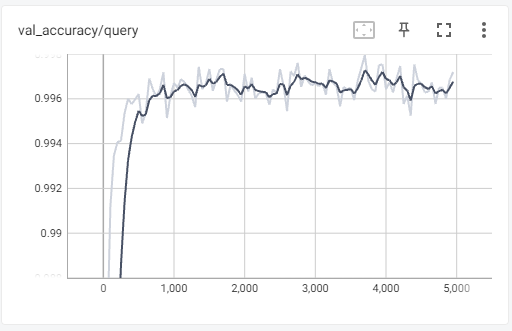
\includegraphics[width=\linewidth]{figures/protonets_validation_query_accuracy.png}
\end{figure}
        
    \end{enumerate}
    
    \newpage
    \item 4 accuracy metrics are logged. For the above run, examine these in detail to reason about what the algorithm is doing.
    \begin{enumerate}[label=(\alph*)]
        \item (5 pt) Is the model placing support examples of the same class close together in feature space or not? Support your answer by referring to specific accuracy metrics.
        
        \textcolor{red}{Model is placing support examples of the same class close together in feature space according to train support accuracy.}

        
        \item (5 pt) Is the model generalizing to new tasks? If not, is it overfitting or underfitting? Support your answer by referring to specific accuracy metrics.
        
        \textcolor{red}{Model is generalizing to new tasks according to validation query accuracy.}

    \end{enumerate}
    
    \newpage
    \item We will now compare different settings at training time. Train on 5-way 1-shot tasks with 15 query examples per task. 
    \begin{enumerate}
        \item (3 pt) Compare your two runs (5-way 1-shot training and 5-way 5-shot training) by assessing test performance on 5-way 1-shot tasks. To assess a trained model on test tasks, run
        \begin{equation*}
            \texttt{python protonet.py --test}
        \end{equation*}
    appropriately specifying \texttt{log\_dir} and \texttt{checkpoint\_step}. Submit a table of your results with 95\% confidence intervals.
        
\begin{tabular}{r|cc}
train                              &5-way 1-shot&5-way 5-shot\\\hline
mean                            &0.986            &0.987            \\ 
95\% confidence interval&0.002            &0.002            \\
\end{tabular}
        
        \item (2 pt) How did you choose which checkpoint to use for testing for each model? 
        
        \textcolor{red}{I chose the latest checkpoint because that will be the most fitted one.}
        
        \item (5 pt) Is there a significant difference in the test performance on 5-way 1-shot tasks? Explain this by referring to the protonets algorithm.
        
        \textcolor{red}{No, computing the prototype is almost the same as choosing one datapoint.}

    \end{enumerate}
    
    

\end{enumerate}



\newpage
\section*{Part 2: Model-Agnostic Meta-Learning (MAML)~\cite{maml}}

\subsubsection*{Algorithm Overview}

\begin{figure}[H]
\centering
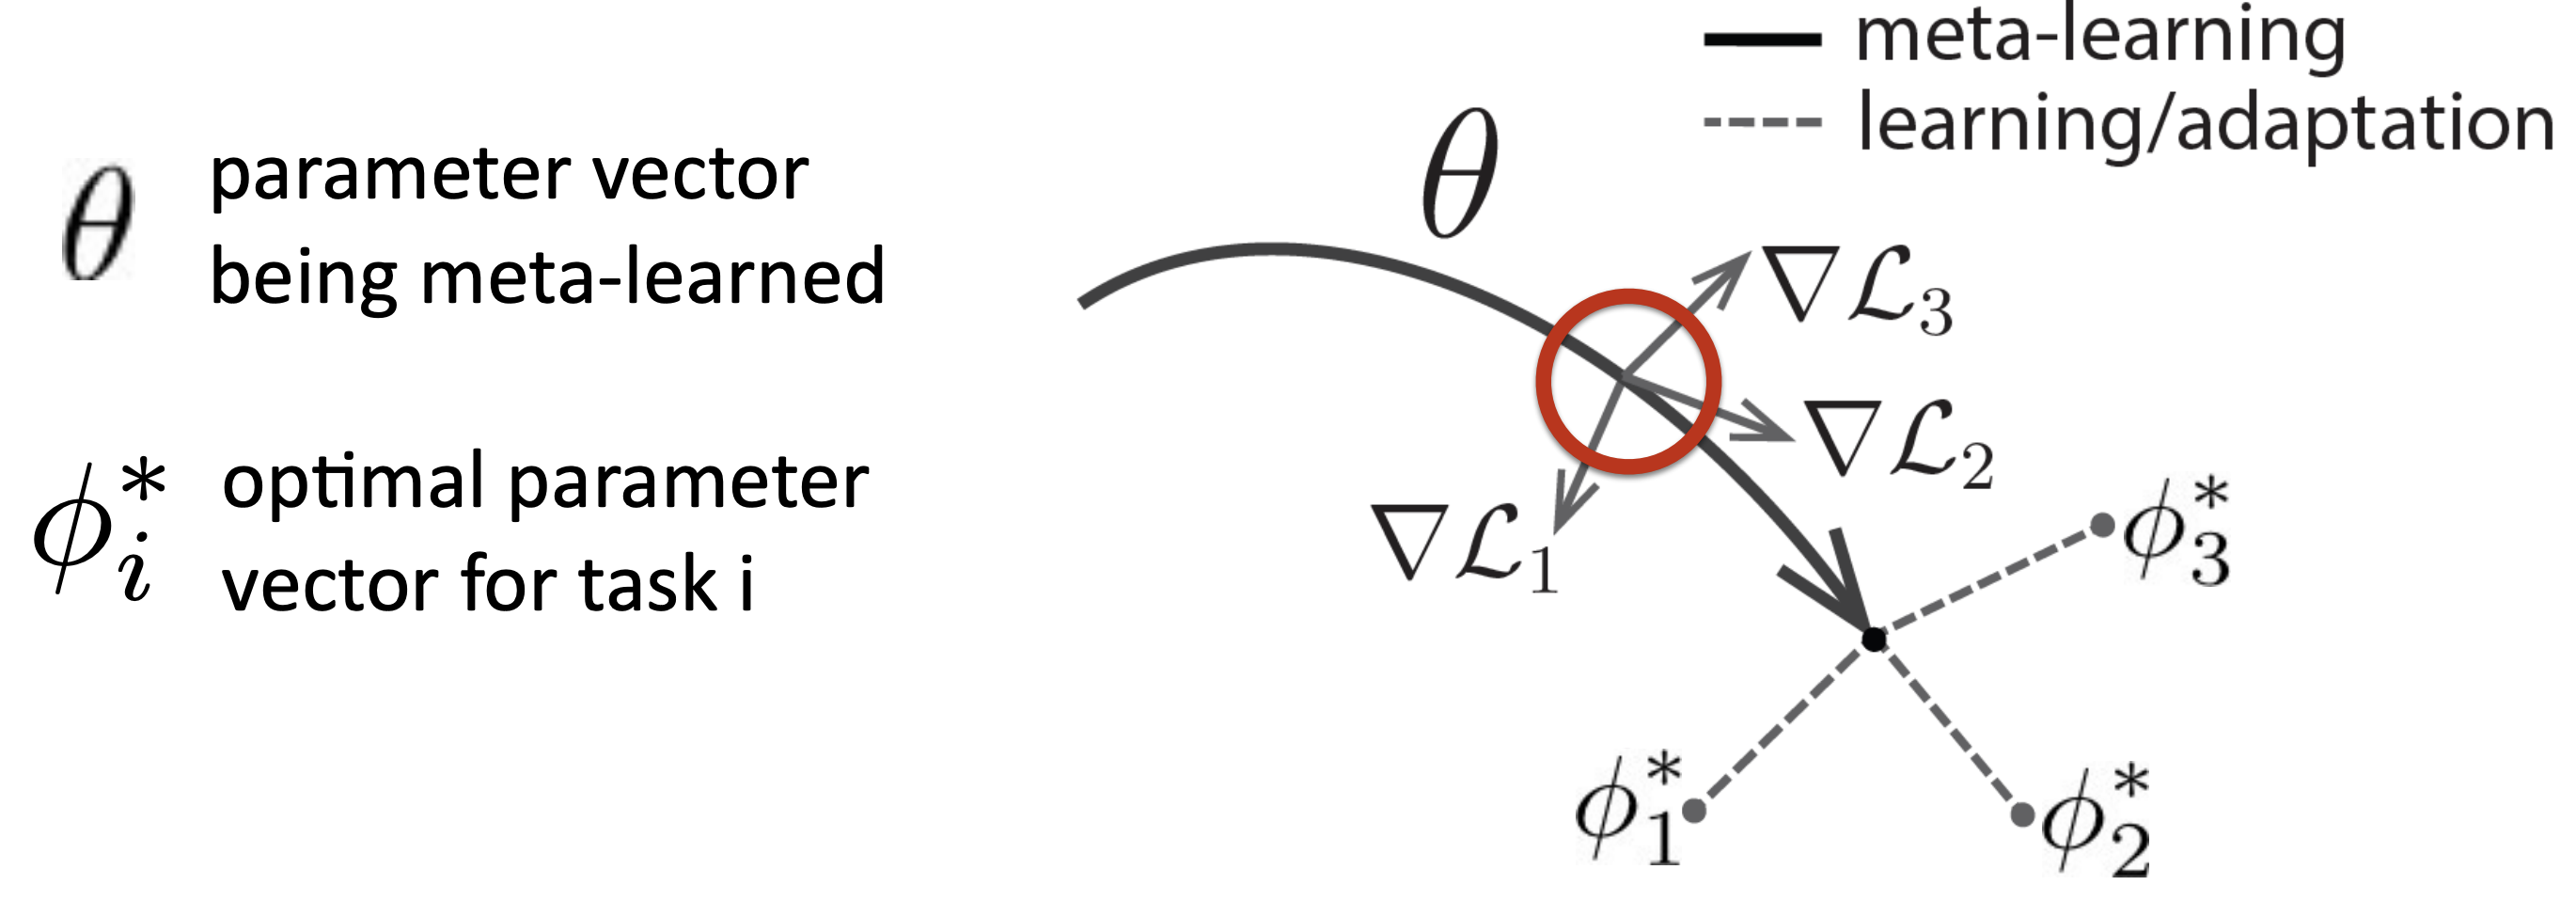
\includegraphics[width=0.8\linewidth]{figures/MAML.png}
\vspace{-3mm}
\caption{MAML in a nutshell. MAML tries to find an initial parameter vector $\theta$ that can be quickly adapted via task gradients to task-specific optimal parameter vectors.}
\label{fig:maml}
\end{figure}

As discussed in lecture, the basic idea of MAML is to meta-learn parameters $\theta$ that can be quickly adapted via gradient descent to a given task. To keep notation clean, define the loss $\mathcal{L}$ of a model with parameters $\phi$ on the data $\dataset_i$ of a task $\task_i$ as
\begin{equation}\label{eq:maml loss}
    \mathcal{L}(\phi, \dataset_i) = \frac{1}{\lvert \dataset_i \rvert} \sum_{(x^j, y^j) \in \dataset_i} -\log p_\phi (y = y^j | x^j)
\end{equation}
Adaptation is often called the \emph{inner loop}. For a task $\task_i$ and $L$ inner loop steps, adaptation looks like the following:
\begin{equation}
\begin{aligned}
    \phi^1 &= \phi^0 - \alpha \nabla_{\phi^0} \mathcal{L}(\phi^0, \supportdata_i) \\
    \phi^2 &= \phi^1 - \alpha \nabla_{\phi^1} \mathcal{L}(\phi^1, \supportdata_i) \\
    \vdots \\
    \phi^L &= \phi^{L-1} - \alpha \nabla_{\phi^{L-1}} \mathcal{L}(\phi^{L-1}, \supportdata_i)
\end{aligned}
\end{equation}
where we have defined $\theta = \phi^0$.


Notice that only the support data is used to adapt the parameters to $\phi^L$. (In lecture, you saw $\phi^L$ denoted as $\phi_i$.) To optimize $\theta$ in the \emph{outer loop}, we use the same loss function~\eqref{eq:maml loss} applied on the adapted parameters and the query data:
\begin{equation}
    \mathcal{J}(\theta) = \E_{\task_i \sim p(\task), (\supportdata_i, \querydata_i) \sim \task_i} \left[ \mathcal{L}(\phi^L, \querydata_i) \right] \label{eq:maml_objective}
\end{equation}


For this homework, we will further consider a variant of MAML~\cite{mamlplusplus} that proposes to additionally learn the inner loop learning rates $\alpha$. Instead of a single scalar inner learning rate for all parameters, there is a separate scalar inner learning rate for each parameter group (e.g. convolutional kernel, weight matrix, or bias vector). Adaptation remains the same as in vanilla MAML except with appropriately broadcasted multiplication between the inner loop learning rates and the gradients with respect to each parameter group. 

The full MAML objective is
\begin{equation}
    \mathcal{J}(\theta, \alpha) = \E_{\task_i \sim p(\task), (\supportdata_i, \querydata_i) \sim \task_i} \left[ \mathcal{L}(\phi^L, \querydata_i) \right] \label{eq:full_objective}
\end{equation}
Like before, we will use minibatches to approximate \eqref{eq:full_objective} and use the Adam optimizer.

\subsubsection*{Problems}


\begin{enumerate}
    \item In the \texttt{maml.py} file, complete the implementation of the \texttt{MAML.\_inner\_loop} and \\ \texttt{MAML.\_outer\_step} methods. The former computes the task-adapted network parameters (and accuracy metrics), and the latter computes the MAML objective (and more metrics). Pay attention to the inline comments and docstrings. \\
    \textbf{Hint}: the simplest way to implement \texttt{\_inner\_loop} involves using \texttt{autograd.grad}. \\
    \textbf{Hint}: to understand how to use the Boolean \texttt{train} argument of \texttt{MAML.\_outer\_step}, read the documentation for the \texttt{create\_graph} argument of \texttt{autograd.grad}.
    
    Assess your implementation of vanilla MAML on 5-way 1-shot Omniglot. Comments from the previous part regarding arguments, checkpoints, TensorBoard, resuming training, and testing all apply. Use 1 inner loop step with a \textbf{fixed} inner learning rate of 0.4. Use 15 query examples per class per task. Do not adjust the outer learning rate from its default of $0.001$. Note that MAML generally needs more time to train than protonets.
    \begin{enumerate}
        \newpage
        \item (20 pt) Submit a plot of the validation post-adaptation query accuracy over the course of training. \\
        \textbf{Hint}: you should obtain a query accuracy on the validation split of at least $96\%$.
        
\begin{figure}[H]
\centering
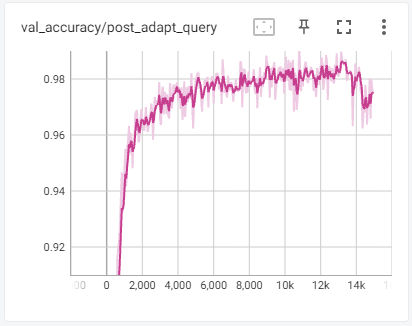
\includegraphics[width=\linewidth]{figures/maml_validation_query_accuracy.png}
\end{figure}
        
    \end{enumerate}
    
    \newpage
    \item 6 accuracy metrics are logged. Examine these in detail to reason about what MAML is doing.
    \begin{enumerate}[label=(\alph*)]
        \item (10 pt) State and explain the behavior of the \texttt{train\_pre\_adapt\_support} and \texttt{val\_pre\_adapt\_support} accuracies. Your answer should explicitly refer to the task sampling process. \\ \textbf{Hint}: consult the \texttt{omniglot.py} file.

        \textcolor{red}{Pre-adapt accuracies are around 0.2 because tasks are randomly sampled.}

    
        \item (5 pt) Compare the \texttt{train\_pre\_adapt\_support} and \texttt{train\_post\_adapt\_support} accuracies. What does this comparison tell you about the model? Repeat for the corresponding \texttt{val} accuracies.

        \textcolor{red}{The model has adapted to the task.}
        
        \item (5 pt) Compare the \texttt{train\_post\_adapt\_support} and \texttt{train\_post\_adapt\_query} accuracies. What does this comparison tell you about the model? Repeat for the corresponding \texttt{val} accuracies.
        
        \textcolor{red}{The model has adapted to the task but did not overfit to data.}

    \end{enumerate}

    \newpage
    \item Try MAML with the same hyperparameters as above except for a fixed inner learning rate of $0.04$.
    \begin{enumerate}[label=(\alph*)]
        \item (3 pt) Submit a plot of the validation post-adaptation query accuracy over the course of training with the two inner learning rates ($0.04$, $0.4$).
        
\begin{figure}[H]
\centering
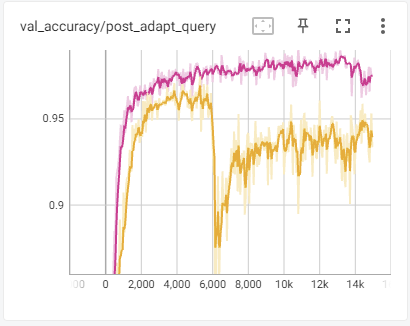
\includegraphics[width=\linewidth]{figures/3a.png}
\end{figure}


        \item (2 pt) What is the effect of lowering the inner learning rate on (outer-loop) optimization and generalization?

        \textcolor{red}{Optimization and generalization failed at one point.}

    \end{enumerate}
    
    \newpage
    \item Try MAML with a fixed inner learning rate of $0.04$ for $5$ inner loop steps.
    \begin{enumerate}[label=(\alph*)]
        \item (3 pt) Submit a plot of the validation post-adaptation query accuracy over the course of training with the two number of inner loop steps ($1$, $5$) with inner learning rate $0.04$.
  
\begin{figure}[H]
\centering
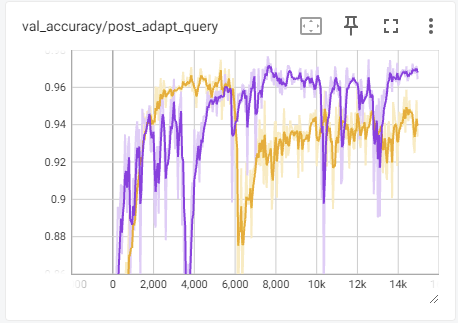
\includegraphics[width=\linewidth]{figures/4a.png}
\end{figure}

        \item (2 pt) What is the effect of increasing the number of inner loop steps on (outer-loop) optimization and generalization?
        
        \textcolor{red}{Optimization and generalization fail more often but recover faster.}

    \end{enumerate}

    \newpage
    \item Try MAML with learning the inner learning rates. Initialize the inner learning rates with $0.4$.
    \begin{enumerate}[label=(\alph*)]
        \item (3 pt) Submit a plot of the validation post-adaptation query accuracy over the course of training for learning and not learning the inner learning rates, initialized at $0.4$. 

\begin{figure}[H]
\centering
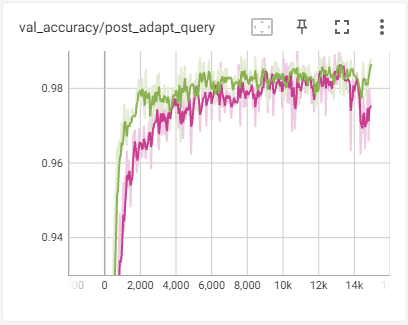
\includegraphics[width=\linewidth]{figures/5a.png}
\end{figure}

        \item (2 pt) What is the effect of learning the inner learning rates on (outer-loop) optimization and generalization?

        \textcolor{red}{Optimization and generalization became more robust.}

    \end{enumerate}
\end{enumerate}

\newpage
\section*{Part 3: More Support Data at Test Time}

In practice, we usually have more than 1 support example at test time. Hence, one interesting comparison is to train both algorithms with $5$-way $1$-shot tasks (as you've already done) but assess them using more shots.

\begin{enumerate}
    \item Use the protonet trained with 5-way 1-shot tasks, and the MAML trained with \textbf{learned} inner learning rates initialized at 0.4. Try $K = 1, 2, 4, 6, 8, 10$ at test time. Use $Q = 10$ for all values of $K$. 
    \begin{enumerate}
        \item (10 pt) Submit a plot of the test accuracies for the two models over these values of $K$ with the 95\% confidence intervals as error bars or shaded regions. 

        \textcolor{red}{Your plot goes here.}

        
        \item (5 pt) How well is each model able to use additional data in a task without being explicitly trained to do so?

        \textcolor{red}{Your answer goes here.}

    \end{enumerate}
\end{enumerate}

\newpage
\section*{A Note}
You may wonder why the performance of these implementations don't match the numbers reported in the original papers. One major reason is that the original papers used a different version of Omniglot few-shot classification, in which multiples of $90^{\degree}$ rotations are applied to each image to obtain 4 times the total number of images and characters. Another reason is that these implementations are designed to be pedagogical and therefore straightforward to implement from equations and pseudocode as well as trainable with minimal hyperparameter tuning. Finally, with our use of batch statistics for batch normalization during test (see code), we are technically operating in the \emph{transductive} few-shot learning setting.

\newpage
\bibliography{references}
\bibliographystyle{unsrt}

\end{document}

